\documentclass[10pt,a4paper]{article}
\usepackage[utf8]{inputenc}
\usepackage[T1]{fontenc}
\usepackage[french]{babel}
\usepackage{lmodern}
\usepackage[margin=1.7cm,top=1.4cm,bottom=1.6cm]{geometry}
\usepackage{graphicx}
\usepackage{booktabs}
\usepackage{tabularx}
\usepackage{enumitem}
\usepackage{caption}
\usepackage[hidelinks]{hyperref}
\usepackage{titlesec}

\setlist{nosep,leftmargin=1.2em}
\titlespacing*{\section}{0pt}{6pt}{3pt}
\titleformat{\section}{\normalsize\bfseries}{\thesection.}{0.4em}{}
\captionsetup{font=small,labelfont=bf,skip=3pt}
\setlength{\parskip}{2pt}
\setlength{\parindent}{0pt}
\newcommand{\nb}[1]{\textbf{#1}}

\begin{document}

\begin{center}
{\large\bfseries Les pénuries de médicaments en France : prévisibles, contagieuses, importées ?}\\[2pt]
{\small DALAS -- TME4 : question de recherche et dataset (version préliminaire) \quad·\quad [Nom 1], [Nom 2] \quad·\quad
\href{https://github.com/OzanTaskin/DALAS_DATASET}{github.com/OzanTaskin/DALAS\_DATASET}}
\end{center}

\section{Questions de recherche}

Depuis 2021, les pénuries de médicaments se multiplient en Europe (amoxicilline, corticoïdes, antiépileptiques…).
Les agences publient la liste des pénuries \emph{en cours}, mais aucune prévision. Nous posons trois questions :

\begin{itemize}
  \item \nb{Question principale (prévisibilité).} Peut-on anticiper les pénuries en France, et quels facteurs rendent une
  substance vulnérable ? Formellement : pour une substance active (code ATC niveau 5) au mois $t$, quelle est la probabilité
  qu'une nouvelle pénurie soit déclarée entre $t+1$ et $t+3$ ? Facteurs envisagés : nombre de laboratoires et de génériques,
  forme (injectable ou orale), volume consommé, criticité officielle, classe thérapeutique, saison, pénuries passées.
  \item \nb{Q1 (contagion entre substituts).} Une pénurie augmente-t-elle le risque de pénurie des autres substances de la
  même classe thérapeutique (ATC niveau 4), vers lesquelles les prescriptions se reportent ?
  \item \nb{Q2 (pénuries importées).} Une pénurie de la même substance en Italie ou en Allemagne annonce-t-elle une pénurie en France ?
\end{itemize}

La France est au centre car c'est le seul pays dont nous avons l'\emph{univers complet} des médicaments commercialisés,
donc aussi ceux qui ne sont jamais en pénurie (indispensable pour prédire). L'Italie et l'Allemagne servent de signaux.
Q1 et Q2 seront testées en comparant un modèle avec et sans les variables « cascade » ou « Europe ».

\section{Collecte des données}

Nous avons construit le dataset à partir de sources officielles publiques (scraping et API), collectées le 05/10/2026 par
un script reproductible. Les fichiers bruts sont conservés sans modification et tracés (URL, date, empreinte SHA-256) ;
une vérification automatique contrôle que rien ne manque. \nb{292 fichiers, 483 Mo.}

\begin{center}\small
\begin{tabularx}{\linewidth}{@{}l l X l@{}}
\toprule
Source & Pays & Contenu & Format \\
\midrule
ANSM, disponibilité des produits de santé & FR & pénuries publiées : statut, dates, médicament, substance & page HTML \\
BDPM (base publique des médicaments) & FR & univers complet : 15\,883 médicaments, boîtes, substances, génériques, MITM & fichiers texte \\
Open Medic (Assurance Maladie) & FR & boîtes remboursées par an (2019-2025), classification ATC complète & CSV (ZIP) \\
AIFA / BfArM & IT / DE & listes de pénuries avec ATC, dates, raisons & CSV \\
EMA ; AEMPS (API CIMA) & UE ; ES & pénuries suivies par l'EMA, liste critique de l'UE ; pénuries espagnoles & JSON, XLSX \\
\bottomrule
\end{tabularx}
\end{center}

\nb{Le problème central est l'historique} : une pénurie terminée disparaît des listes. Pour reconstruire le passé, nous avons
récupéré les \nb{archives mensuelles de la Wayback Machine} (Internet Archive) : 58 archives de la page ANSM (04/2021--09/2026),
47 de la liste italienne (10/2021--09/2026), 12 de la liste allemande (07/2024--09/2026) et 132 de la BDPM (2015--2026), qui
permettent de décrire le marché tel qu'il était connu à chaque date et d'éviter les fuites d'information.

\section{Description quantitative}

Le dataset est organisé autour d'une table centrale, \texttt{shortage\_events} : \nb{une ligne = un épisode de pénurie d'un
médicament dans un pays} (pays, médicament, substance, ATC5, ATC4, début, fin, en cours, gravité, criticité, raison).
Elle compte \nb{17\,343 épisodes}, décrits par des tables sur les médicaments, la classification ATC et la consommation.

\begin{center}\small
\begin{tabular}{@{}l r r r r l@{}}
\toprule
Pays & Épisodes de pénurie & En cours & Substances (ATC5) & ATC connu & Période observée \\
\midrule
France (ANSM) & 1\,599 & 180 & 551 & 95\,\% & 04/2021--10/2026 \\
Italie (AIFA) & 10\,998\textsuperscript{*} & 2\,169 & 1\,051 & 94\,\% & 10/2021--10/2026 \\
Allemagne (BfArM) & 1\,319 & 404 & 410 & 97\,\% & 07/2024--10/2026 \\
\bottomrule
\end{tabular}\\[1pt]
{\footnotesize \textsuperscript{*} hors 3\,427 arrêts définitifs de commercialisation, qui ne sont pas des pénuries.}
\end{center}

\begin{figure}[h]
\centering
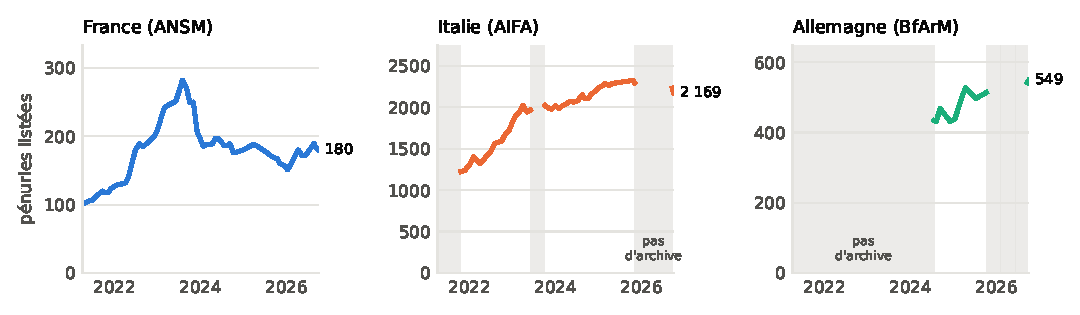
\includegraphics[width=\linewidth]{figures/evolution_penuries.pdf}
\caption{Nombre de pénuries listées dans chaque archive. Zones grises : pas d'archive disponible (la courbe est interrompue).
Échelles différentes par pays : les agences ne recensent pas les pénuries de la même façon.}
\end{figure}

\vspace{-4pt}
\begin{minipage}[t]{0.47\linewidth}
\vspace{0pt}
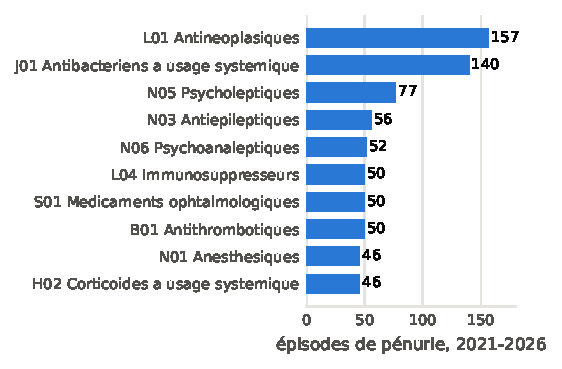
\includegraphics[width=\linewidth]{figures/classes_france.pdf}
\captionof{figure}{Les 10 classes thérapeutiques (ATC niveau 2) les plus touchées en France.}
\end{minipage}\hfill
\begin{minipage}[t]{0.5\linewidth}
\vspace{0pt}\small
\textbf{France.} Les nouvelles pénuries publiées passent de 311 (2022) à \nb{350 (2023)}, pic de la crise des antibiotiques
de l'hiver 2022-2023, puis 264 (2024) et 185 (2025). 60\,\% sont des tensions d'approvisionnement, 40\,\% des ruptures.
Durée médiane : \nb{128 jours} (quartiles 53 et 284 jours, 1\,130 épisodes complets) ; 18\,\% durent plus d'un an.
Anticancéreux et antibiotiques dominent (fig.~2).

\textbf{Univers de prédiction.} 13\,650 médicaments commercialisés, dont 81\,\% ont un code ATC, soit 1\,539 substances :
\nb{551 (36\,\%) ont connu au moins une pénurie} depuis 2021. Consommation : environ 2,3 milliards de boîtes remboursées
par an (19 à 27 milliards d'euros, 2019-2025).

\textbf{Signal européen.} 384 des 551 substances françaises en pénurie l'ont aussi été en Italie ou en Allemagne.
Raisons déclarées en Italie : problèmes de production (37\,\%), forte demande (10\,\%).
\end{minipage}

\section{Prétraitement et choix}

Les données passent par trois niveaux : \emph{brut} (fichiers inchangés), \emph{nettoyé} (16 tables Parquet, une ligne =
un objet), puis \emph{final} (panel substance × mois, à construire après le cours \emph{ML Protocol}). Principaux choix :

\begin{itemize}
  \item \nb{Classification ATC.} Ni l'ANSM ni la BDPM ne la donnent. Nous l'obtenons par Open Medic, la liste MITM ou un
  médicament aux mêmes substances. Les 1\,470 fiches ANSM sont rapprochées par lien exact BDPM (808), nom (246), substance (126)
  ou marque (203) : 94\,\% ont un ATC5 ; la méthode utilisée est conservée.
  \item \nb{Épisodes.} Les observations mensuelles sont regroupées en épisodes. La date affichée par l'ANSM est une date de
  mise à jour : à la première apparition d'une fiche, elle tombe entre deux archives dans 98,5\,\% des cas et sert de date de
  début, remplacée par la date exacte de la BDPM quand elle existe (556 épisodes). Un retour en pénurie après une remise à
  disposition est un nouvel épisode.
  \item \nb{Exclusions.} Arrêts définitifs de commercialisation (Italie) ; codes ATC invalides ; épisodes déjà en cours en
  avril 2021 signalés pour ne pas biaiser les durées.
\end{itemize}

\textbf{Limites.} (1) La page ANSM ne liste que les pénuries communiquées publiquement (surtout les médicaments d'intérêt
thérapeutique majeur) : notre cible est ce sous-ensemble. (2) Les archives sont irrégulières : une pénurie apparue et résolue
entre deux archives peut être manquée, et la liste italienne n'a aucune archive entre 11/2025 et 09/2026, période où l'AIFA
a retiré environ 1\,500 entrées anciennes. (3) Les définitions de pénurie diffèrent selon les pays, et les obligations de
déclaration ont été renforcées : une partie de la hausse est un effet de déclaration. (4) L'Espagne n'est pas encore
intégrée (l'API ne fournit pas l'ATC).

\end{document}
